% =============================================================
% Experiment 1
% Clipping and Clamping Circuits using Diodes
%
% Required packages in the master document preamble:
%   amsmath, amssymb, graphicx, circuitikz, pgfplots, booktabs,
%   enumitem, siunitx, hyperref
%   \pgfplotsset{compat=1.17}
% =============================================================

\chapter{Experiment 1(b): Clamping Circuits using Diodes}
\label{sec:expt1}

\section{Aim}
\begin{enumerate}[label=(\roman*)]
	\item To study the operation of positive and negative clamping circuits.
	\item To design and test clamper circuits for specified output requirements.
	%\item To verify, using a DSO, that the observed waveforms agree with the theoretically predicted transfer characteristics.
\end{enumerate}
\section{Pre-Lab Exercise}
Before performing the experiment, simulate the circuits and verify the designs using LTspice or any other circuit simulation software. 
\section{Equipment/Components Required}
\begin{table}[h!]
	\centering
	\begin{tabular}{@{}cll@{}}
		\toprule
		S.No. & Equipment/Component & Specification \\
		\midrule
		1 & Digital Storage Oscilloscope & 2-channel, 20--50\,MHz bandwidth \\
		2 & Function Generator\footnote{Instead of function generator, a step-down transformer may also be used to apply the input signal, which will then be a 50 Hz sine wave.} & Sine wave, 1\,Hz -- 1\,MHz \\
		3 & Regulated DC Power Supply & 0--30\,V \\
		4 & Silicon diode & 1N4007 (or equivalent), 2 nos. \\
	%	5 & Zener diodes & $V_z$ = 5.6 V, 2 nos. \\
		5 & Resistors & 1\,k$\Omega$ -- 100\,k$\Omega$ \\
		6 & Capacitors & 1\,$\mu$F -- 10\,$\mu$F \\
		7 & Breadboard and connecting wires & -- \\
		\bottomrule
	\end{tabular}
	\caption{Equipment and component list.}
\end{table}

\section{Theory}

A \emph{clamper} shifts the entire waveform up or down without altering its shape, thereby changing its DC reference level.

Throughout this document, the diode is modelled as an ideal switch in series with a cut-in voltage $V_F \approx 0.7\,\text{V}$ (silicon) and a forward resistance $R_f \approx 0$; the reverse resistance is assumed infinite. 

A clamper consists of a diode, a capacitor, and a resistor, arranged so that the capacitor charges (through the low forward resistance of the diode) to the peak of the input during one half-cycle and holds this charge (discharging slowly through $R_L$, with $R_LC \gg T$) during the rest of the cycle, thereby shifting the DC level of the waveform. It essentially `clamps' the input signal up or down by the peak voltage. It is also called a DC restorer.

Mathematically, for an input signal given by $v){in}(t) = V_m\sin(\omega t)$, the clamper output is $v_o(t)= \pm V_m + V_m\sin(\omega t)$.

\paragraph{(a) Negative Clamper.}
Figure~\ref{fig:neg_clamper} shows a negative clamper, which shifts the waveform downward so that its positive peak is clamped at (approximately) $0\,\text{V}$ (or at $V_F$, accounting for diode drop).

\begin{figure}[htbp]
	\centering
	\begin{subfigure}{0.4\textwidth}
		\centering
		\begin{circuitikz}[american, scale=1.20, line width = 0.85pt]
			\draw
			(0,0) to[sinusoidal voltage source, l=$v_{in}(t)$] (0,3)
			(0,3) to[cC, name = C, l=$C$, *-*] (2,3)
			(2,3) to[short] (3.5,3)
			(2,3) to[D, l=$D$, *-, mirror] (2,0)
			(2,0) to[short, -*] (0,0)
			(3.5,3) to[R, l=$R_L$] (3.5,0)
			(3.5,0) to [short, -*] (2,0);	
			\node [above left=1pt] at (C.left){\small $+$};	
		\end{circuitikz}
		\caption{Negative clamper circuit.}
		\label{fig:neg_clamper}
	\end{subfigure}
	\begin{subfigure}{0.52\textwidth}
		\centering
		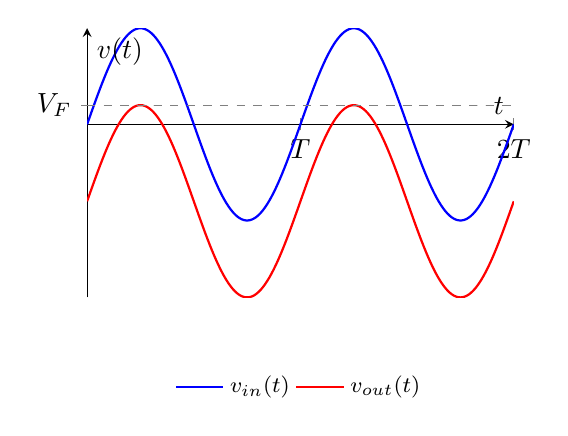
\begin{tikzpicture}
			\begin{axis}[
				width=7cm, height=5cm,
				xlabel={$t$}, 
				ylabel={$v(t)$},
				ylabel style={
					at={(axis description cs:0,1)},  % top-left corner of the axis
					anchor=south,
					rotate=90,
				},
				axis lines=middle,
				ymin=-4.5, ymax=2.5,
				xtick={0,1,2},
				xticklabels={$0$,$T$,$2T$},
				ytick={0.5},
				yticklabels={$V_F$},
				domain=0:2, samples=200,
				legend style={draw=none, font=\footnotesize, at={(0.5,-0.25)}, anchor=north, legend columns=2}
				]
				\addplot[blue, thick] {2.5*sin(360*x)};
				\addlegendentry{$v_{in}(t)$}
				\addplot[red, thick] {2.5*sin(360*x) - 2.5 + 0.5};
				\addlegendentry{$v_{out}(t)$}
				\addplot[gray, dashed] {0.5};
			\end{axis}
		\end{tikzpicture}
		\caption{Input and output waveforms for the negative clamper.}
		\label{fig:negWave_clamper}
	\end{subfigure}
	\caption{Negative Clamper: Circuit and waveforms}
\end{figure}

\paragraph{(b) Positive Clamper.}
Reversing the diode polarity (Figure~\ref{fig:pos_clamper}) clamps the negative peak of the waveform at approximately $0\,\text{V}$, shifting the entire waveform upward.

\begin{figure}[htbp]
	\centering
	\begin{subfigure}{0.42\textwidth}
		\centering
		\begin{circuitikz}[american, scale=1.0, line width=0.85pt]
			\draw
			(0,0) to[sinusoidal voltage source, l=$v_{in}(t)$] (0,3)
			(0,3) to[cC, name = C, l=$C$, invert, *-*] (2,3)
			(2,3) to[short] (3.5,3)
			(2,3) to[D, l=$D$, *-, invert] (2,0)
			(2,0) to[short, -*] (0,0)
			(3.5,3) to[R, l=$R_L$] (3.5,0)
			(3.5,0) to [short, -*] (2,0);	
			\node [above right=1pt] at (C.left){\small $+$};	
		\end{circuitikz}
		\caption{Positive clamper circuit (diode polarity reversed with respect to Figure~\ref{fig:neg_clamper}).}
		\label{fig:pos_clamper}
	\end{subfigure}
	\begin{subfigure}{0.52\textwidth}
		\centering
		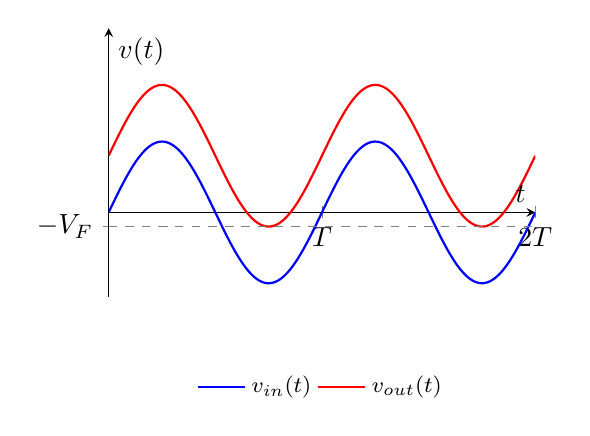
\begin{tikzpicture}
			\begin{axis}[
				width=7cm, height=5cm,
				xlabel={$t$}, 
				ylabel={$v(t)$},
				ylabel style={
					at={(axis description cs:0,1)},  % top-left corner of the axis
					anchor=south,
					rotate=90,
				},
				axis lines=middle,
				ymin=-3, ymax=6.5,
				xtick={0,1,2},
				xticklabels={$0$,$T$,$2T$},
				ytick={-0.5},
				yticklabels={$-V_F$},
				domain=0:2, samples=200,
				legend style={draw=none, font=\footnotesize, at={(0.5,-0.25)}, anchor=north, legend columns=2}
				]
				\addplot[blue, thick] {2.5*sin(360*x)};
				\addlegendentry{$v_{in}(t)$}
				\addplot[red, thick] {2.5*sin(360*x) + 2.5 - 0.5};
				\addlegendentry{$v_{out}(t)$}
				\addplot[gray, dashed] {-0.5};
			\end{axis}
		\end{tikzpicture}
		\caption{Input and output waveforms for the positive clamper.}
		\label{fig:posWaveClamper}
	\end{subfigure}
	\caption{Positive clamper: Circuit and waveforms}
\end{figure}
For an input sine wave of amplitude $V_m$, the steady-state clamped output ideally swings between:
\begin{align}
	\text{Negative clamper: } && v_{out} &\in [-2V_m + V_F,\; V_F], \label{eq:neg_clamp}\\
	\text{Positive clamper: } && v_{out} &\in [-V_F,\; 2V_m - V_F]. \label{eq:pos_clamp}
\end{align}
The time constant $R_L C$ must satisfy $R_L C \gg T$ (the input period) so that the capacitor voltage does not decay appreciably between successive charging peaks (poor choice of $R_L C$ leads to \emph{waveform tilt/sag}).
%\clearpage
\section{Circuit Diagrams}
The circuits are as shown in the previous sections.
\begin{notebox}
	While preparing the lab-report, circuit diagrams shall contain proper labels for the components, including the component part numbers (such as 1N4001), and values/parameters (example: $10\ V_{pp}$, Sine, 100 Hz, for the source; $R_1$, $1\ \text{k}\Omega$, etc.).
\end{notebox}	
\section{Design Example}
\begin{enumerate}[label=(\alph*)]
	\item Select the operating signal's frequency and amplitude, $V_m = 10\ \text{V}$ and $f = 100\ \text{Hz}$. 
	\item The series resistor R should not be too large or too small. $R_{min}$ is decided by the maximum current in the circuit. A typical value for R would be $1\ \text{k}\Omega$. Since $R_L\gg R$, $R_L \geq 100\ \text{k}\Omega$\footnote{For viewing on the DSO, $R_L$ may be removed, then $V_{out}$ would be same as $V_{in}$, since the input impedance of DSO is in $\text{M}\Omega$.  In practical circuits where the clipped waveform is applied as input to other circuits, $R_L$ represents the input impedance of those circuits.}. The output voltage peak then would be:
	\[
	V_{out,m}=\frac{V_mR_L}{R+R_L} = \frac{10\times 100\ \text{k}}{1\ \text{k}+100\ \text{k}} = 9.9 \ \text{V}
	\]
	
	\item For a \textbf{biased clipper} required to clip at a level $V_{clip}$, select $V_R = V_{clip} - V_F$ using a potential divider from the DC supply, or a battery/regulated source directly. A Zener diode may also be chosen, as described earlier. Let $V_{clip} = 6.3\ \text{V}$. Then $V_R = V_{clip} - V_F\ =\ 6.3-0.7 = 5.6\ \text{V}$. In this case, either a dc voltage of $5.6\ \text{V}$ or a Zener diode of $V_Z=5.6\ \text{V}$ may be used as bias $V_R$.
	\item For a \textbf{clamper}, choose $C$ such that $R_L C \geq 10\,T$, where $T = 1/f$ is the period of the lowest input frequency to be used, so that the sag in output during discharge is limited to within an acceptable fraction (typically $< 5\%$) of $V_m$. For $f=100\ \text{Hz}$, $T=10\ \text{ms}$. Then, for $C = 1\ \mu F$ electrolytic:
	\[
	R_L C \geq 10\,T \Rightarrow R_L \geq \frac{10\times 10\times 10^{-3}}{1\times 10^{-6}}
	\], which yields:
	\[
	R_L\geq 100\ \text{k}\Omega
	\]
	%\item Choose $R_L$ in clampers large enough to limit diode conduction current to a safe value. 
	\item \textbf{Selection of diodes}: For input frequencies less than 1 kHz, line frequency diodes such as 1N4001 may be used. For higher frequencies, these slow diodes are to be replaced with faster signal diodes such as 1N4148.
\end{enumerate}
%\begin{notebox}
%	Show the actual design in the lab report instead of reproducing the design procedure.
%\end{notebox}
\section{Experiment Procedure}

\begin{enumerate}[label=\arabic*.]
	\item Assemble the shunt positive clipper of Figure~\ref{fig:shunt_pos_clipper} on the breadboard. Set the function generator to a sine wave of frequency $1\,\text{kHz}$ and amplitude $10\,\text{V}_{pp}$. 
	\item Connect DSO CH1 to $v_{in}$ and CH2 to $v_{out}$, with a common ground. Display both waveforms simultaneously and sketch/record them.
	\item Replace the shunt positive clipper with the shunt negative clipper. (Figure~\ref{fig:shunt_neg_clipper}). Record $v_{in}$ and $v_{out}$, and measure the clipping level from the DSO screen using the horizontal cursors.
	\item Repeat for the biased clipper (Figure~\ref{fig:biased_clipper}) for at least two values of $V_R$, and the double clipper (Figure~\ref{fig:double_clipper}). (\emph{Note that the peak of the selected input waveform is to be higher than the clipping level for the case of biased clippers}).
	\item For each clipper configuration, tabulate the theoretically expected and experimentally measured clipping levels.
	\item Assemble the negative clamper (Figure~\ref{fig:neg_clamper}) using the design values of $R_L$ and $C$ computed in the Design Procedure. Apply the same sine wave and record $v_{in}$ and $v_{out}$ on the DSO, noting the DC shift and any tilt/sag in the output.
	\item Repeat for the positive clamper (Figure~\ref{fig:pos_clamper}).
	\item For each clamper, measure $V_{out,max}$ and $V_{out,min}$ using DSO cursors and compare with Equations~\eqref{eq:neg_clamp}--\eqref{eq:pos_clamp}.
	\item Vary the input frequency (e.g., to $100\,\text{Hz}$) while keeping $R_L C$ fixed, and observe/record the effect on clamper output tilt. Explain the observation.
\end{enumerate}

\section{Precautions}
\begin{itemize}
	\item Observe correct diode polarity while assembling each circuit; an inverted diode produces the mirror-image (and often misleading) result.
	\item Do not exceed the diode's maximum forward current or reverse voltage ratings (Important if you are using a step-down transformer to give the input signal (50 Hz), instead of a function generator).
	\item Ensure a common ground between the function generator and both DSO channels.
	%	\item For clamping circuits, allow a few cycles for the capacitor to reach steady-state charge before recording the output.
	\item Electrolytic capacitors, if used, connect with correct polarity as per the expected DC level at that node.
\end{itemize}
\section{Expected Waveforms}
The sample waveforms for the clipping circuits are as shown in Figs.~\ref{fig:wavePosClipper}, \ref{fig:waveNegClipper},\ref{fig:biasedClipperWaves}, \ref{fig:biasedNegClipperWaves} and \ref{fig:slicerWaves}. The waveforms for the clamping circuits are as shown in Figs.~\ref{fig:negWave_clamper}, ~\ref{fig:posWaveClamper}. When recording waveforms, note down all the salient points/features of the waveforms, such as voltage/time details.

\section{Observation Tables}
The observation table for the clipping circuits is given in Table~\ref{tab:ObsClippers}. Use Table~\ref{tab:ObsClampers} to tabulate the Clamper circuit observations.
\begin{table}[ht!]
	\centering
	\begin{tabular}{@{}lccccc@{}}
		\toprule
		Circuit & $V_{clip}$ (theory) & $V_{clip}$ (measured) & \% Error \\
		\midrule
		Shunt positive clipper &  &  &  \\
		Shunt negative clipper &  &  &  \\
		Biased positive clipper ($V_{R1}$) &  &  &  \\
		Biased megative clipper ($V_{Z}$) &  &  &  \\
		Double clipper (upper level) &  &  &  \\
		Double clipper (lower level) &  &  &  \\
		\bottomrule
	\end{tabular}
	\caption{Clipping circuits: theoretical vs. measured clipping levels.}
	\label{tab:ObsClippers}
\end{table}

\begin{table}[ht!]
	\centering
	\begin{tabular}{@{}lcccc@{}}
		\toprule
		Circuit & $V_{out,max}$ (theory) & $V_{out,max}$ (meas.) & $V_{out,min}$ (theory) & $V_{out,min}$ (meas.) \\
		\midrule
		Negative clamper &  &  &  &  \\
		Positive clamper &  &  &  &  \\
		\bottomrule
	\end{tabular}
	\caption{Clamping circuits: theoretical vs. measured output extremes.}
	\label{tab:ObsClampers}
\end{table}
\section{Results}
\begin{enumerate}
	\item The diode-based clipping circuits with and without external bias are set-up and the output waveforms were studied. 
	\item The diode-based clamping circuits were set-up and the waveforms were studied.
\end{enumerate}


\begin{explorebox}
	Experiment with higher frequency signals. What do you observe? Can you explain why circuit performance is not as expected at higher frequencies?
\end{explorebox}
\section{Questions}
\begin{enumerate}[label=Q\arabic*.]
	\item Distinguish between series and shunt clipper configurations in terms of output impedance and loading effects.
	\item Derive the expression for the clipping level of the biased clipper of Figure~\ref{fig:biased_clipper} in terms of $V_R$ and $V_F$.
	\item Why must the time constant $R_L C$ of a clamper be much greater than the period of the input waveform? What happens if $R_L C$ is comparable to $T$?
	\item Sketch the output waveform of the double clipper (Figure~\ref{fig:double_clipper}) for an input triangular wave of amplitude greater than $(V_{R1}+V_{R2}+2V_F)$.
	\item A clamper is required to shift a $10\,\text{V}_{pp}$, $1\,\text{kHz}$ sine wave so that its output never goes negative. Design suitable values of $R_L$ and $C$, assuming a maximum permissible sag of $2\%$.
	\item Explain why a clipper is sometimes called a \emph{limiter} and give one practical application each of a clipper and a clamper in electronic systems.
	\item Why do clipper circuits do not perform as intended when diodes like 1N4001 are used, at higher frequencies, such as 50 kHz?
\end{enumerate}